\chapter{Aufgaben Erweiterung}
Patrick Niepel \& Marcel Hagmann \& Carl Philipp Knoblauch

\section{Einleitung}
Unsere erste Aufgabe war die Erweiterung der Stundenlpan App um ein Aufgaben Feature. Mit dem Aufgaben Feature kann der Nutzer seine Aufgaben aus Vorlesungen in die App eintragen, die dann mit dem Kalender synchronisiert werden.

\newpage
\section{Planung und Mockup}

Zuallererst machten wir uns Gedanken darüber, welche Informationen der Nutzer beim Hinzufügen seiner Aufgaben in der App angeben muss und möchte. Anhand dieser Erkenntnisse, fertigten wir das Mockup an.


\begin{figure}[ht]
	\centering
  \frame{ 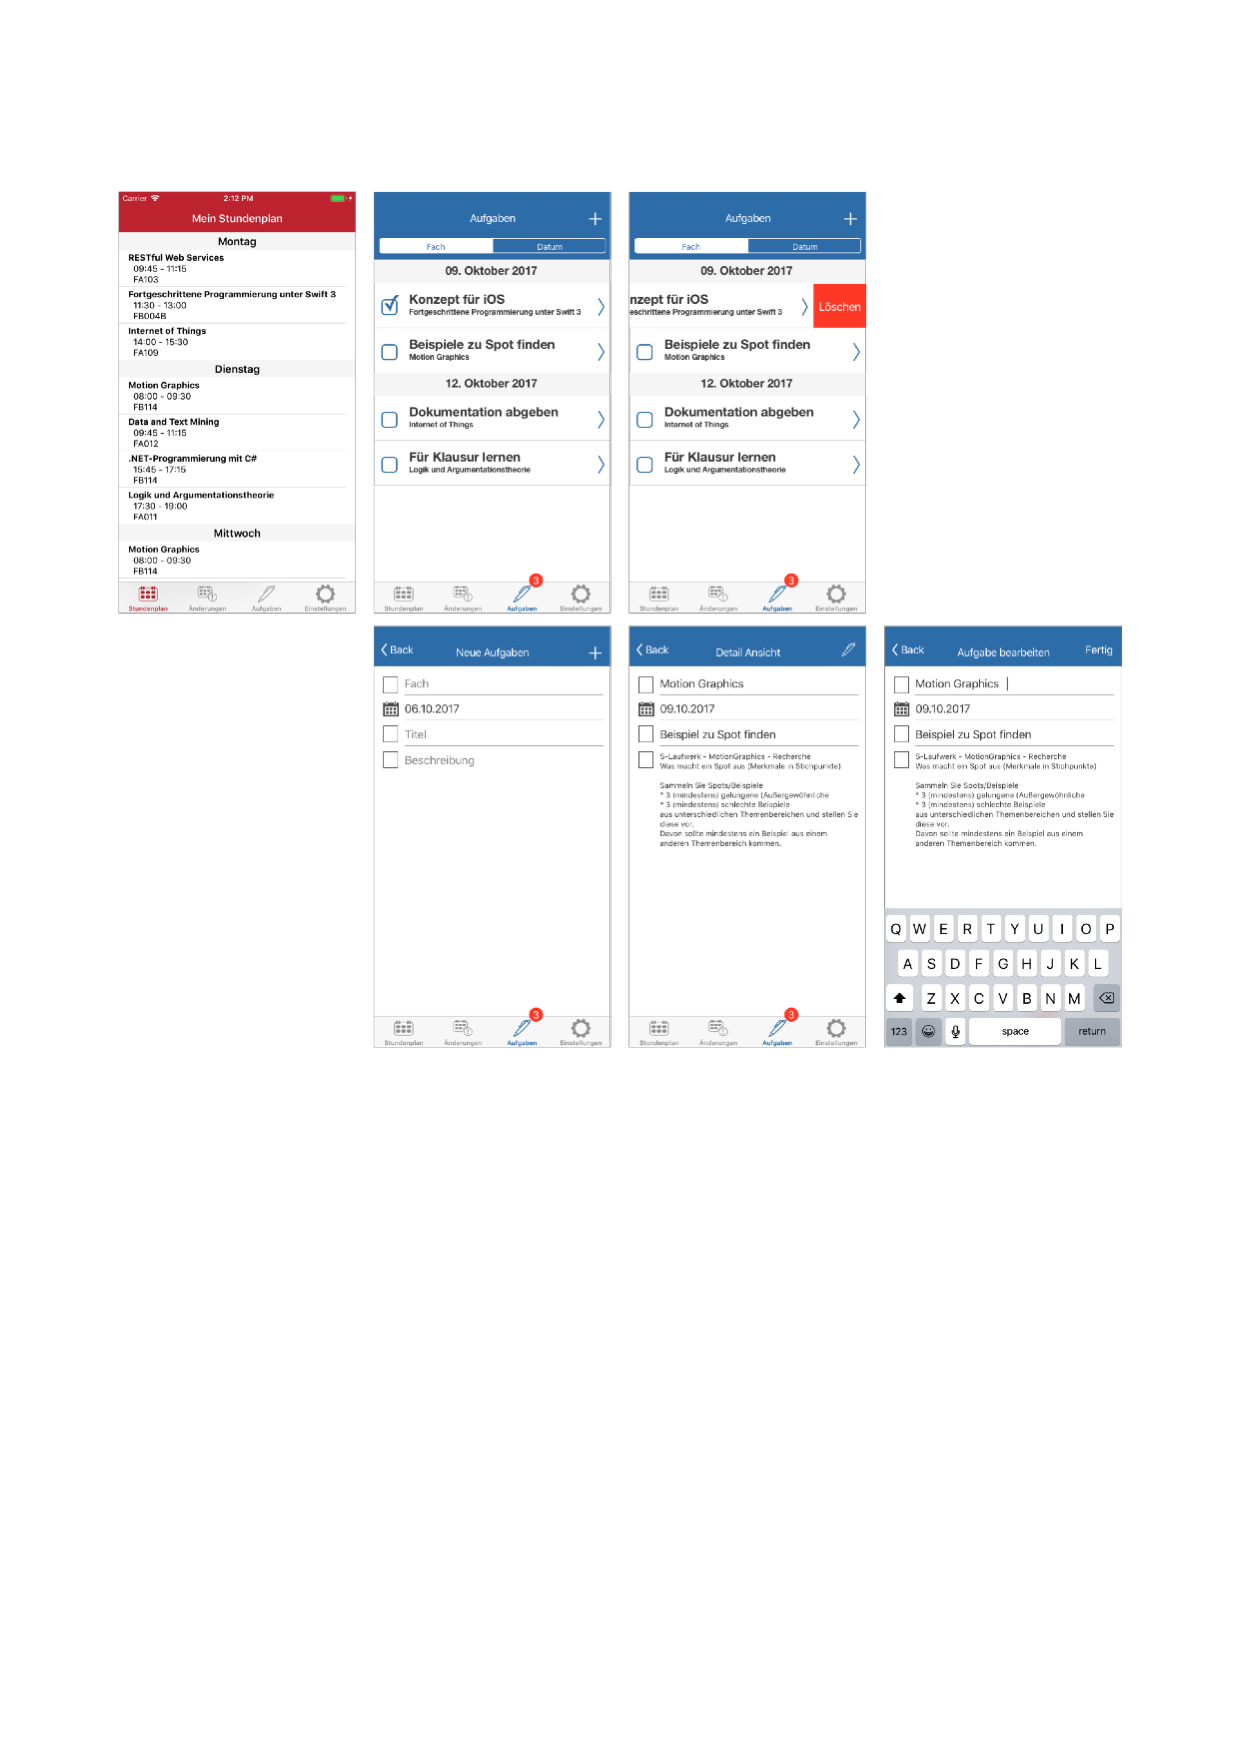
\includegraphics[width=0.9\textwidth]{Mockup_ios_aufgaben} }
	\caption{Mockup unserer Aufgaben Erweiterung}
	\label{fig1}
\end{figure}

\newpage
\section{Funktionen}
\begin{itemize}
\item Sortierung nach Datum und Fach
\item Hinweis der noch zu erledigenden Aufgaben mit einem Badge in der Tab-Bar
\item Hinzufügen, Löschen und Bearbeiten einer Aufgabe
\item Vorlesungen in der Wochenübersicht, denen eine Aufgabe zugeteilt wurde hervorheben
\item Aufgabe mit dem Kalender synchronisieren
\item Speichern der Aufgaben in UserData
\end{itemize}


